\begin{example2}[\quad \large Nem leválasztott érzékelők 2.]

Egy árammérő söntellenellás jellemzői: $Rs=10\;m\Omega{}$, $Ls=0.1\;\mu{}H$. Tervezzen illesztőáramkört, amely a $0..5\;A$ mérési tartományt az AD váltó bemenetére közel frekvenciafüggetlen módon $0..5\;V$-os tartományba alakítja! A sönt 4 kivezetéses, főáramköri negatív pontja közös a jelfeldolgozó elektronika nulla pontjával.

\end{example2}

A feladatban egy árammérő söntöt kell egyfelől jelillesztenünk, másfelől pedig frekvencia kompenzálnunk. Az alábbi kapcsolási rajzra lesz szükségünk:

\begin{figure}[h!]
    \centering
    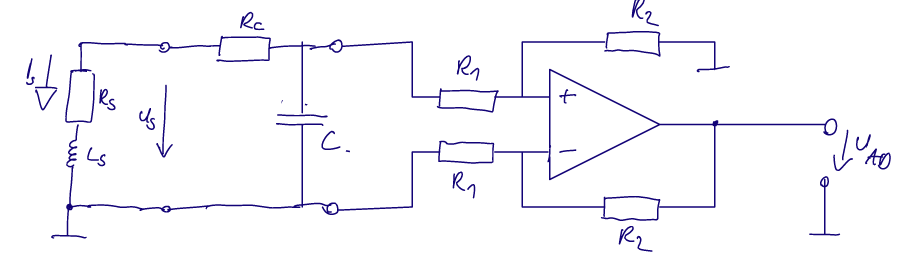
\includegraphics[width=1\linewidth]{Figures//tmp/42_schematic.png}
    \caption{Söntös árammérés mérőerősítővel}
    \label{fig:enter-label}
\end{figure}

1. lépésben határozzuk meg a szükséges erősítési paramétereket. Ehhez kiszámoljuk, hogy az áram mekkora feszültséget ejt az ellenálláson:

\begin{equation}
\begin{aligned}{}
    U_{s} &= R_s \cdot I_s = 10\; m\Omega{} \cdot 5\;A = \underline{50\; mV} \\
\end{aligned}
\end{equation}

Ebből pedig meg tudjuk határozni, hogy mekkora $G$ erősítésre lesz szükségünk:

\begin{equation}
\begin{aligned}{}
    G &= \frac{U_{AD}}{U_S} = \frac{5\;V}{50\;mV} = \underline{100} \\
\end{aligned}
\end{equation}

Innen pedig következnek a mérőerősítő kapcoslás ellenállás értékei. $R_1$-et válasszuk meg $10\;k\Omega$ értéknek.

\begin{equation}
\begin{aligned}{}
    G &= \frac{R_2}{R_1} \\
    R2 &= G \cdot R_1 = 100 \cdot 10\;k\Omega = \underline{1\;M\Omega} \\
\end{aligned}
\end{equation}

Ezek után már csak a sönt ellenállás parazita induktivitásának kompenzálása van hátra:


\begin{equation}
\begin{aligned}{}
    R_C \cdot C &= \frac{L_s}{R_s} \\
    C &= \frac{L_S}{R_S \cdot \R_C} = \frac{0,1\;\mu{H}}{10\;m\Omega \cdot 10\;\Omega} = \underline{1\;nFn} \\
\end{aligned}
\end{equation}